\documentclass[tikz, border=3.14mm]{standalone}
\usepackage{pgfplots}
\pgfplotsset{compat=1.18}
\usepgfplotslibrary{groupplots}

\begin{document}
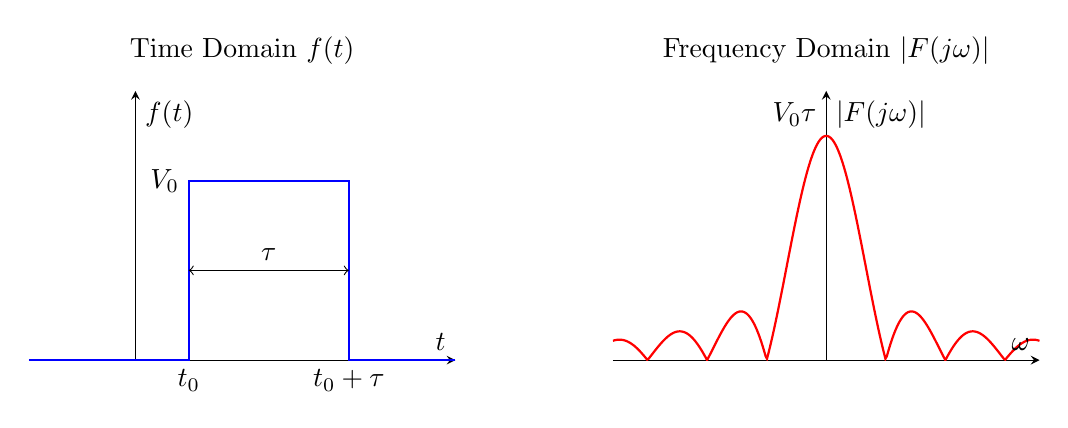
\begin{tikzpicture}
    \begin{groupplot}[
        group style={group size=2 by 1, horizontal sep=2cm},
        axis lines = middle,
        width = 7cm, height = 5cm,
        ymin = 0, ytick = \empty,
        xtick = \empty
    ]
        % Time Domain
        \nextgroupplot[
            title = {Time Domain $f(t)$},
            xlabel = {$t$},
            ylabel = {$f(t)$},
            xmin = -1, xmax = 3,
            ymax = 1.5,
            clip = false
        ]
        \draw[thick, blue] (-1,0) -- (0.5,0) -- (0.5,1) -- (2,1) -- (2,0) -- (3,0);
        \node[anchor=north] at (axis cs:0.5, 0) {$t_0$};
        \node[anchor=north] at (axis cs:2, 0) {$t_0 + \tau$};
        \node[anchor=east] at (axis cs:0.5, 1) {$V_0$};
        \draw[<->] (axis cs:0.5, 0.5) -- node[above] {$\tau$} (axis cs:2, 0.5);

        % Frequency Domain
        \nextgroupplot[
            title = {Frequency Domain $|F(j\omega)|$},
            xlabel = {$\omega$},
            ylabel = {$|F(j\omega)|$},
            xmin = -15, xmax = 15,
            ymax = 1.2,
            samples = 300
        ]
        \addplot[thick, red, domain=-15:15] {abs(sin(deg(x*1.5/2))/(x*1.5/2))};
        \node[anchor=south east] at (axis cs:0, 1) {$V_0 \tau$};
        \node[anchor=north] at (axis cs:4.18, 0) {$\frac{2\pi}{\tau}$};
        \node[anchor=north] at (axis cs:-4.18, 0) {$-\frac{2\pi}{\tau}$};

    \end{groupplot}
\end{tikzpicture}
\end{document}
